\chapter{Background}
\section{Merkle tree \cite{merkle1988digital}}
Ralph Merkle invented the merkle trees in 1979. We present here the binary merkle tree used in bitcoin. We present also a derivation of the patricia tree used in ethereum in \ref{merkle:ethereum}.
\subsection{Binary merkle tree}
\begin{figure}[H]
    \centering
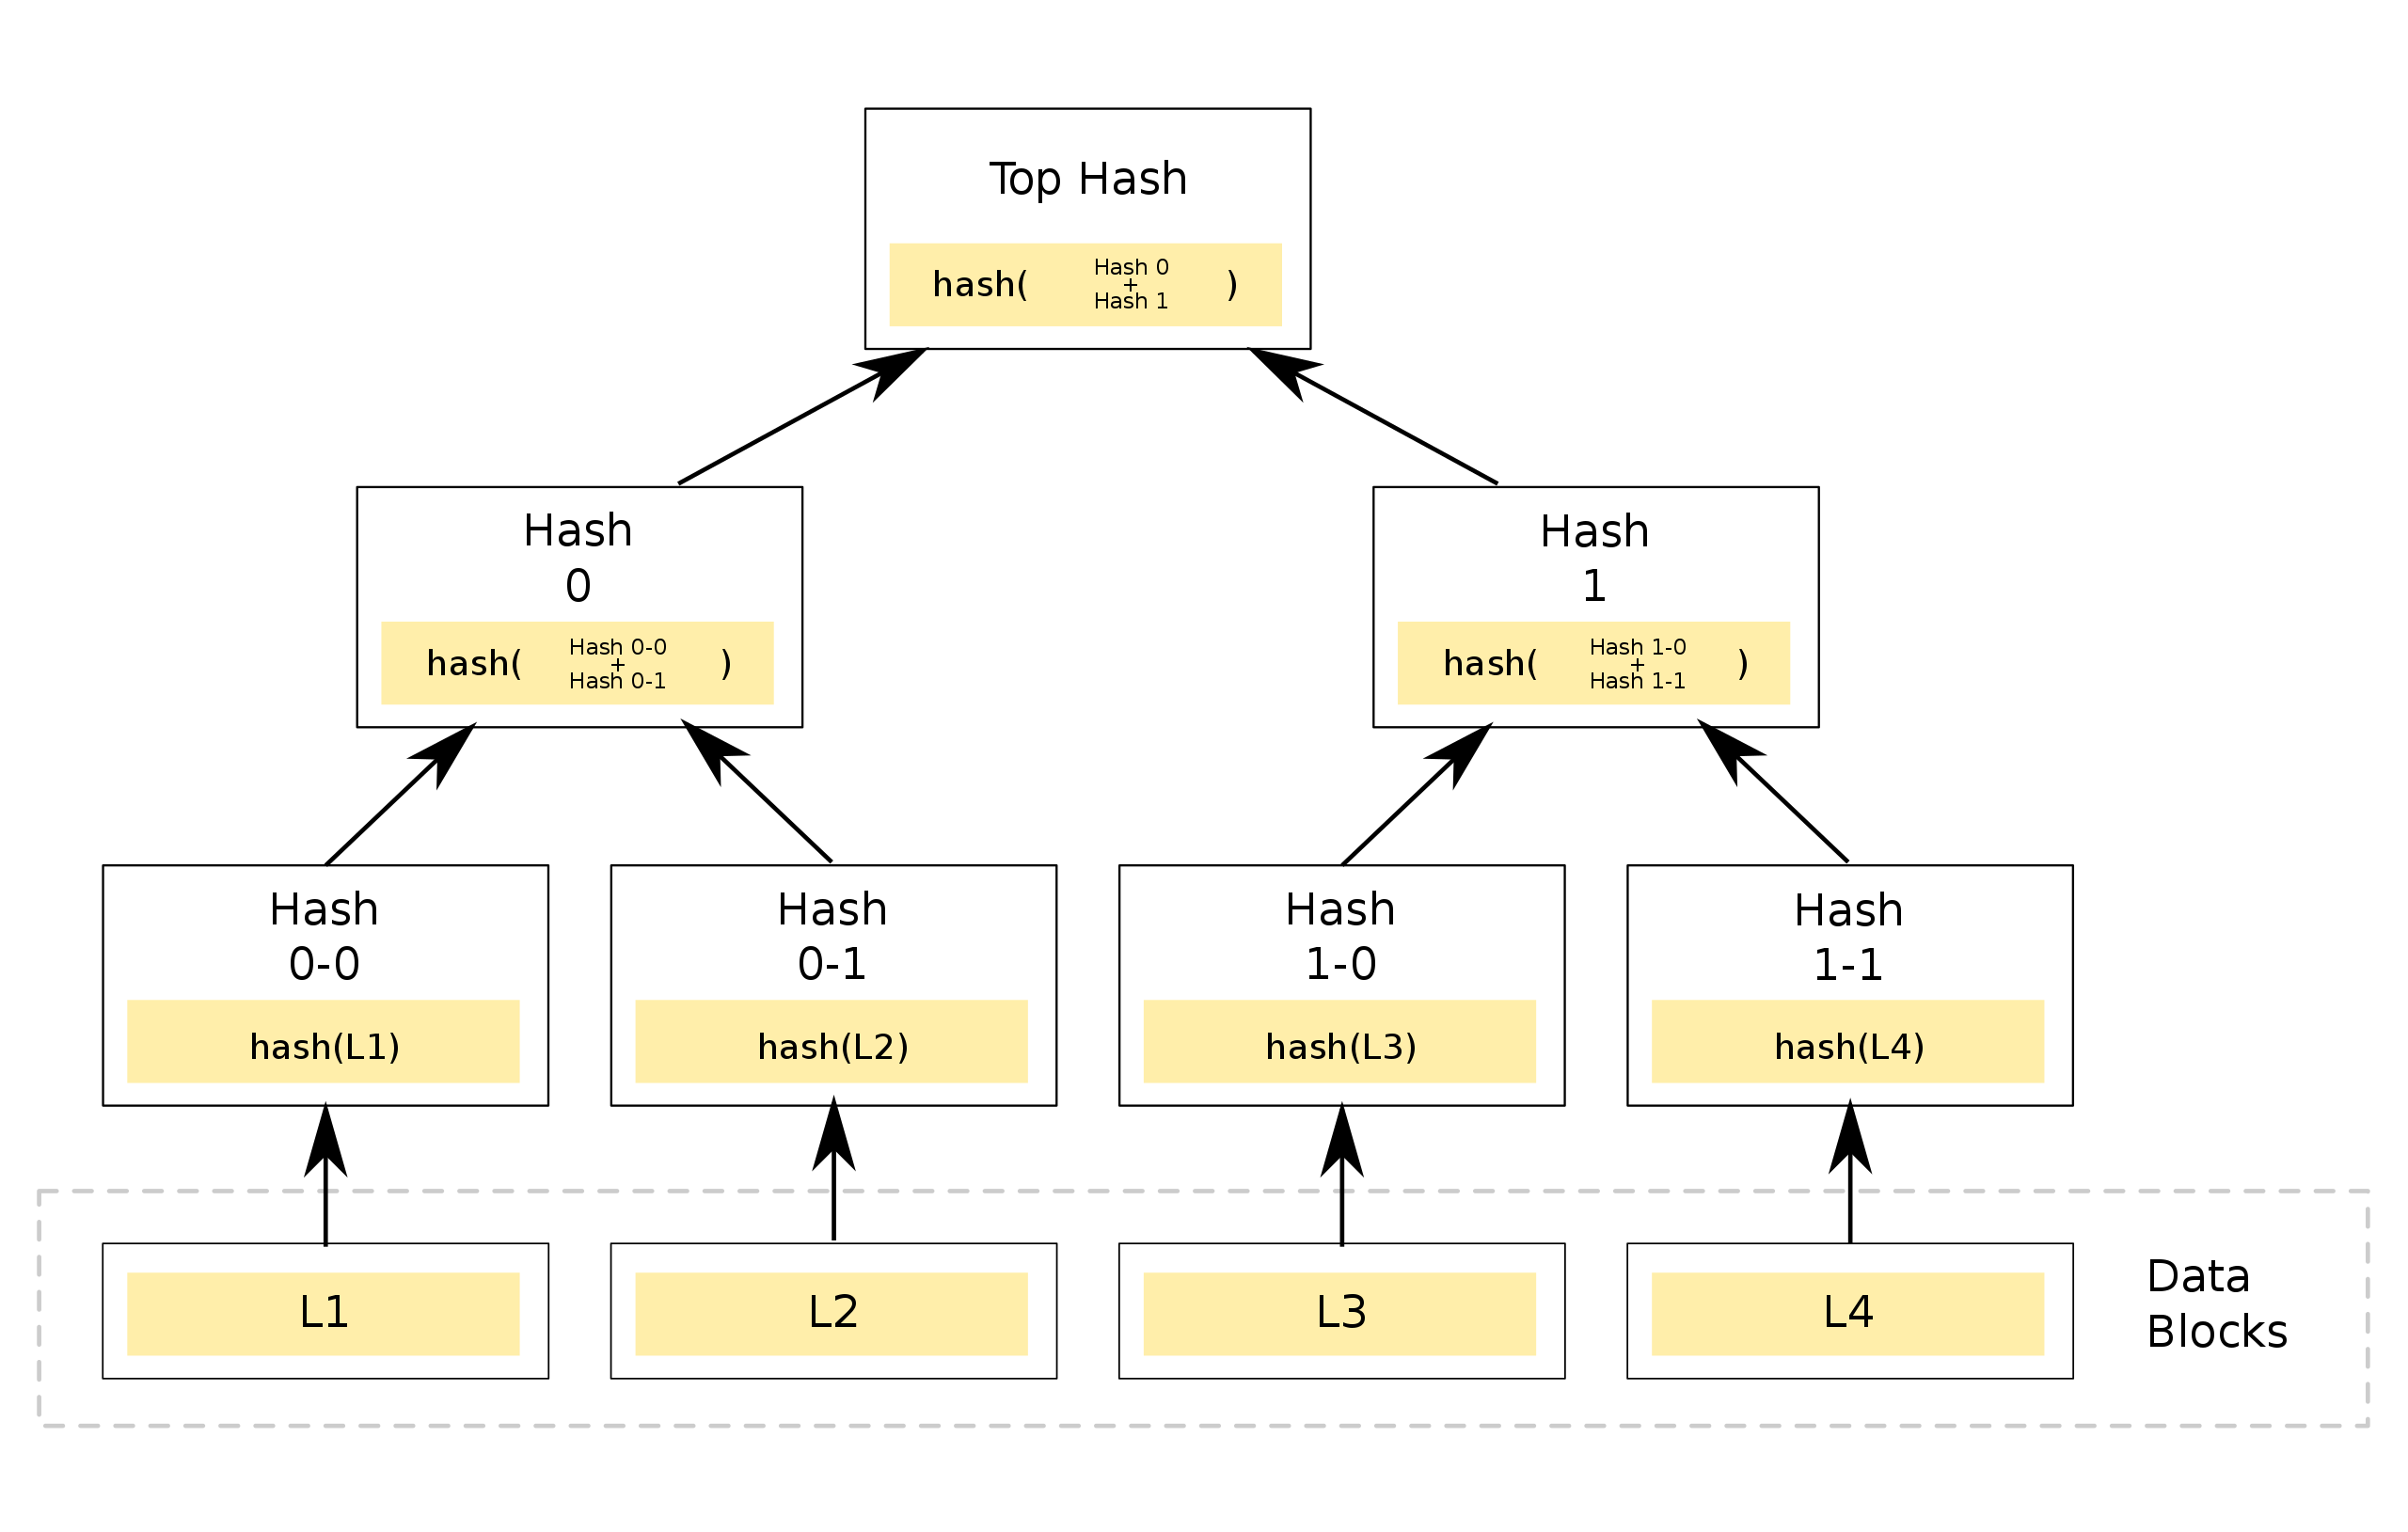
\includegraphics[width=0.7\linewidth]{background/merkle.png}
    \caption{Binary merkle tree}
    \label{fig:merkle}
\end{figure}
The binary merkle tree consists of hashing the transaction two by two: 
\begin{enumerate}
    \item List all the data you want to save in an ordered list: it can be n users for example or any kind of data. In blockchain, these data are the transactions. Here say we have 4 transactions L1, L2, L3, L4.
    \item Hash these data one by one to obtain n hashes. Here we obtain 4 transactions hashes \\($Hash_{0-0},Hash_{0-1},Hash_{1-0},Hash_{1-1})$
    \item Hash the hashes two by two starting from the left. If there is only one node on the right of the tree, we duplicate it two obtain the parent. Here we obtain $Hash_0, Hash_1$.
    \item Repeat the last step until we obtain only one node left: the root.
\end{enumerate}
The root is a fingerprint of all the data, in our case the four transactions. 
It means that if you change anything in the original data, the timestamp of the first transaction for example, it'll change completely the root hash of the merkle tree, thanks to the non locality property of the hash function used (Alice and Aline have very different hashes even if they have only one different letter)

To better understand we'll take an example of a bitcoin merkle tree for the block \href{https://www.blockchain.com/explorer/fr/explorer/blocks/btc/000000000000030de89e7729d5785c4730839b6e16ea9fb686a54818d3860a8d}{170 861}:

\begin{figure}[H]
    \centering
\begin{tikzpicture}
\tikzset{edge from parent/.style={draw,edge from parent path={(\tikzparentnode.south)-- +(0,-8pt)-| (\tikzchildnode)}}}
\Tree 
[.acb5aeb
[.e2d23ad
[.8e45845 [.338bbd0 ] [.1ad1138 ] ]
[.85b994b [.c77834d ] [.bb3d833 ] ] ]
[.13f0f97
[.e2c81be [.38d563c ] [.8fc0507 ] ]
[.9511f44 [.9db9fe6 ] [.3c72fdb ] ] ] ]
\end{tikzpicture}
    \caption{Merkle tree of the bitcoin block \href{https://blockchair.com/bitcoin/block/170861}{170 861}}
    \label{fig:merkletree}
\end{figure}

\subsection{Proof of inclusion} \label{merkle:inclusion}
\iffalse
  \begin{forest}
    for tree={
      edge={{Stealth[]}-},
    }
    [acb5aeb
      [e2d23ad
        [8e45845
          [338bbd0]
            [1ad1138]
            ]
            [85b994b
                [\colorbox{lime}{c77834d}]
                [bb3d833]
            ]
            ]
    [13f0f97
    [e2c81be
    [38d563c] [8fc0507]][9511f44 [9db9fe6][3c72fdb]]]
            ]
  \end{forest}
\fi

Merkle trees allow to summarize the data into one fixed length fingerprint, the root hash. 
But why should we use this data structure instead of just hashing all the hashes for example?

This data structure allows proof of inclusion. In the case of bitcoin for example, data is the transactions, and this structure allows other users to answer this question: \\
\textbf{Is this transaction really included in that block?}

So let's consider the merkle tree below from our example:


\begin{figure}[H]
    \centering
\begin{tikzpicture}
\tikzset{edge from parent/.style={draw,edge from parent path={(\tikzparentnode.south)-- +(0,-8pt)-| (\tikzchildnode)}}}
\Tree 
[.acb5aeb
[.e2d23ad
[.\colorbox{lime}{8e45845} [.338bbd0 ] [.1ad1138 ] ]
[.85b994b [.\colorbox{yellow}{c77834d} ] [.\colorbox{lime}{bb3d833} ] ] ]
[.\colorbox{lime}{13f0f97}
[.e2c81be [.38d563c ] [.8fc0507 ] ]
[.9511f44 [.9db9fe6 ] [.3c72fdb ] ] ] ]
\end{tikzpicture}
    \caption{Proof of inclusion: Transaction to be verified in yellow, merkle proof in green}
    \label{fig:merkleproof}
\end{figure}


We have 8 transaction hashes that we want to place in the merkle tree in this example. Let's say we are interested in the transaction in yellow (c77834d) because it's destinated to our account. We want a proof that this transaction has really happened, and have been included in that block with merkle root acb5aeb. 

The proof is a merkle block with the green hashes. The verifier of this proof can then follow these steps:
\begin{enumerate}
    \item With yellow transaction and the green one bb3d833 you can concatenate and hash it to get the parent hash 85b994b.
    \item With this last hash 85b994b and the green one 8e45845 you can concatenate and hash them to get the parent hash e2d23ad.
    \item And with this last hash concatened with the last green one 13f0f97 and hashed, we get the merkle root
    \item We compare the calculated merkle root from the proof and the real one from the block. If they match, the proof is accepted.
    In bitcoin, it means that the transaction is included in this block. If they don't , we cannot prove the inclusion with that proof. 
\end{enumerate} 
\subsection{Proof scaling}
\textbf{
What is the advantage of using this data structure?}

The verifier only needs the merkle root of the block to accept the proof of inclusion. But as this is a binary tree, the number of hashes at each level is divided by two, so this proof only consists of $\log_2(n)$ hashes, with n the number of transactions. 
It means that if we have 8 transactions, as in this example we  need one hash per level so $\log_2(8)=3$ hashes to proof the inclusion of the transaction in the block.

\colorbox{lime}{
\textbf{
If $n=100$ we need $\log_2(100)\sim 7$ hashes, if $n=1000$ we need $\log_2(1000)\sim 10$ hashes.
}
}

Now there is a trade off. You can reduce the height of the tree by making it wider. Instead of two childs and the binary tree from bitcoin, we can have 16 childs like in Ethereum. This has a drawback as it increase the length of the proof. 
\begin{figure}[H]
    \centering
    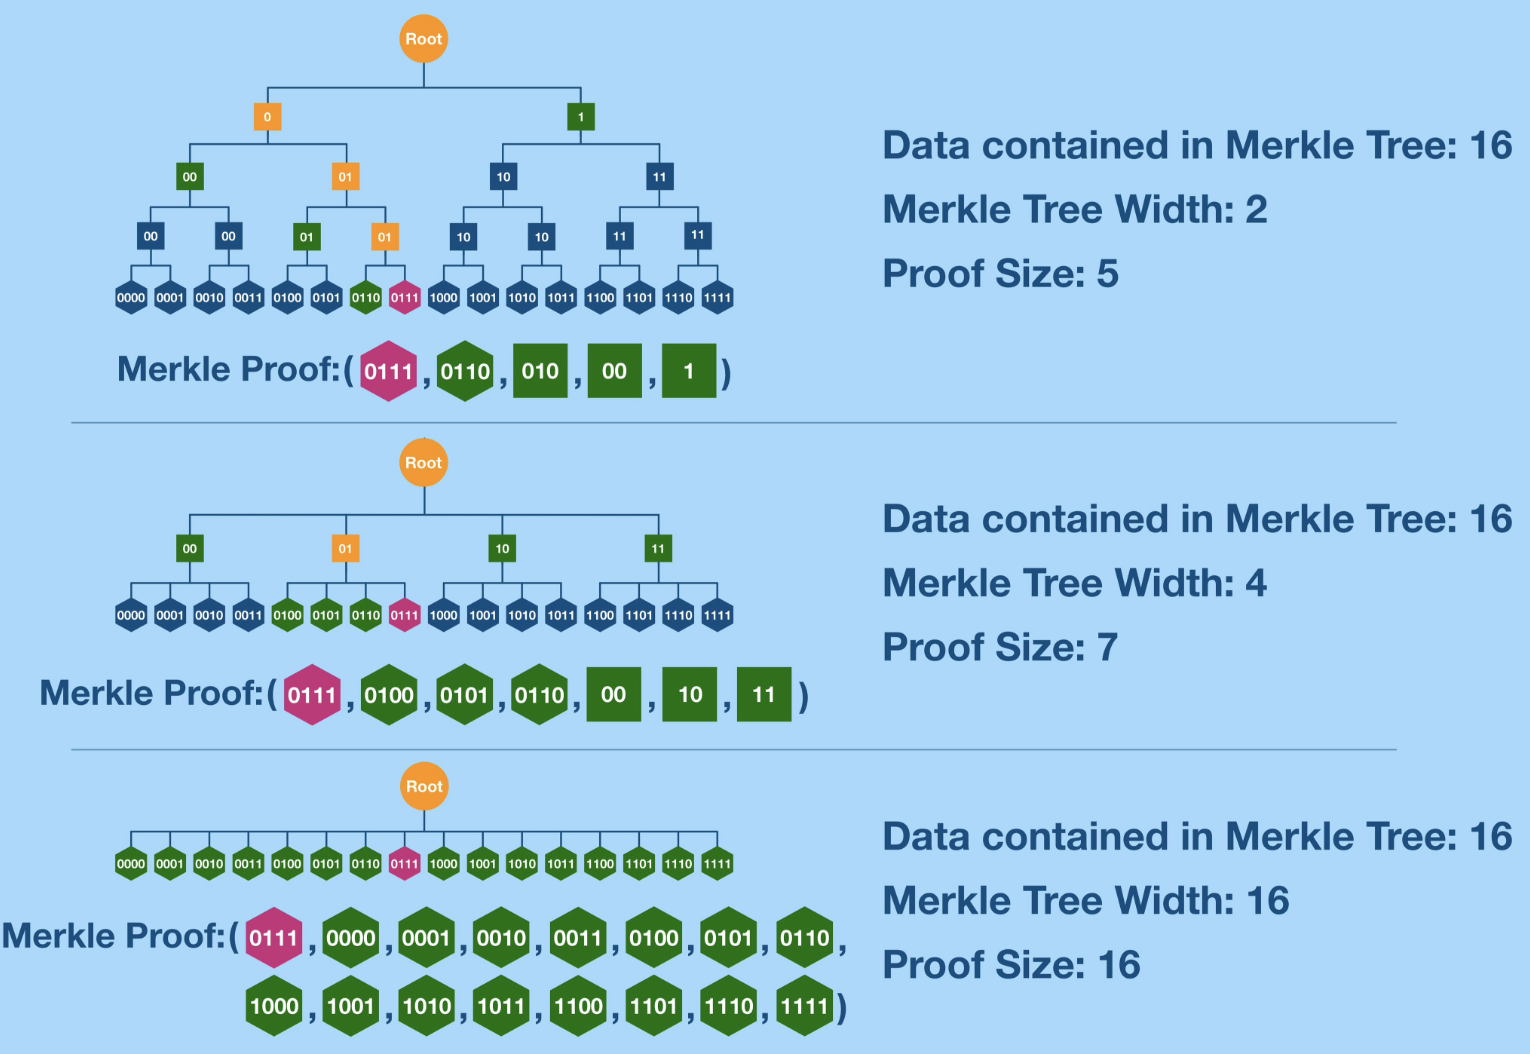
\includegraphics[width=0.7\linewidth]{background/merklescaling.png}
    \caption{Merkle tree proof scaling}
    \label{fig:merklewidth}
\end{figure}

The general formula for calculating the proof's length is $length_{proof}=(m-1)\log_m(n)$ with n leaves of width m.

In general 
Verkle trees \cite{verkle} are an interesting solution to this problem.

\subsection{Some applications}
\textbf{Merkle trees play a key role in distributed systems} because the same data should exist in multiple places. Here the data integrity property is important.

\textbf{Blockchains} since the white paper use the merkle trees to represent data. This allow data integrity as for any distributed systems but also allow the light node to just download the fingerprint of the data.  

\textbf{\cite{sismo} manage groups of accounts} represented in merkle trees. Accounts are a key value pair, the key is the identifier, usually the address of the user, and the value depends on the group. The groups are for example the twitter accounts where the value is the number of followers, or the github contributors where the value is the number of commits. 
\begin{figure}[H]
    \centering
    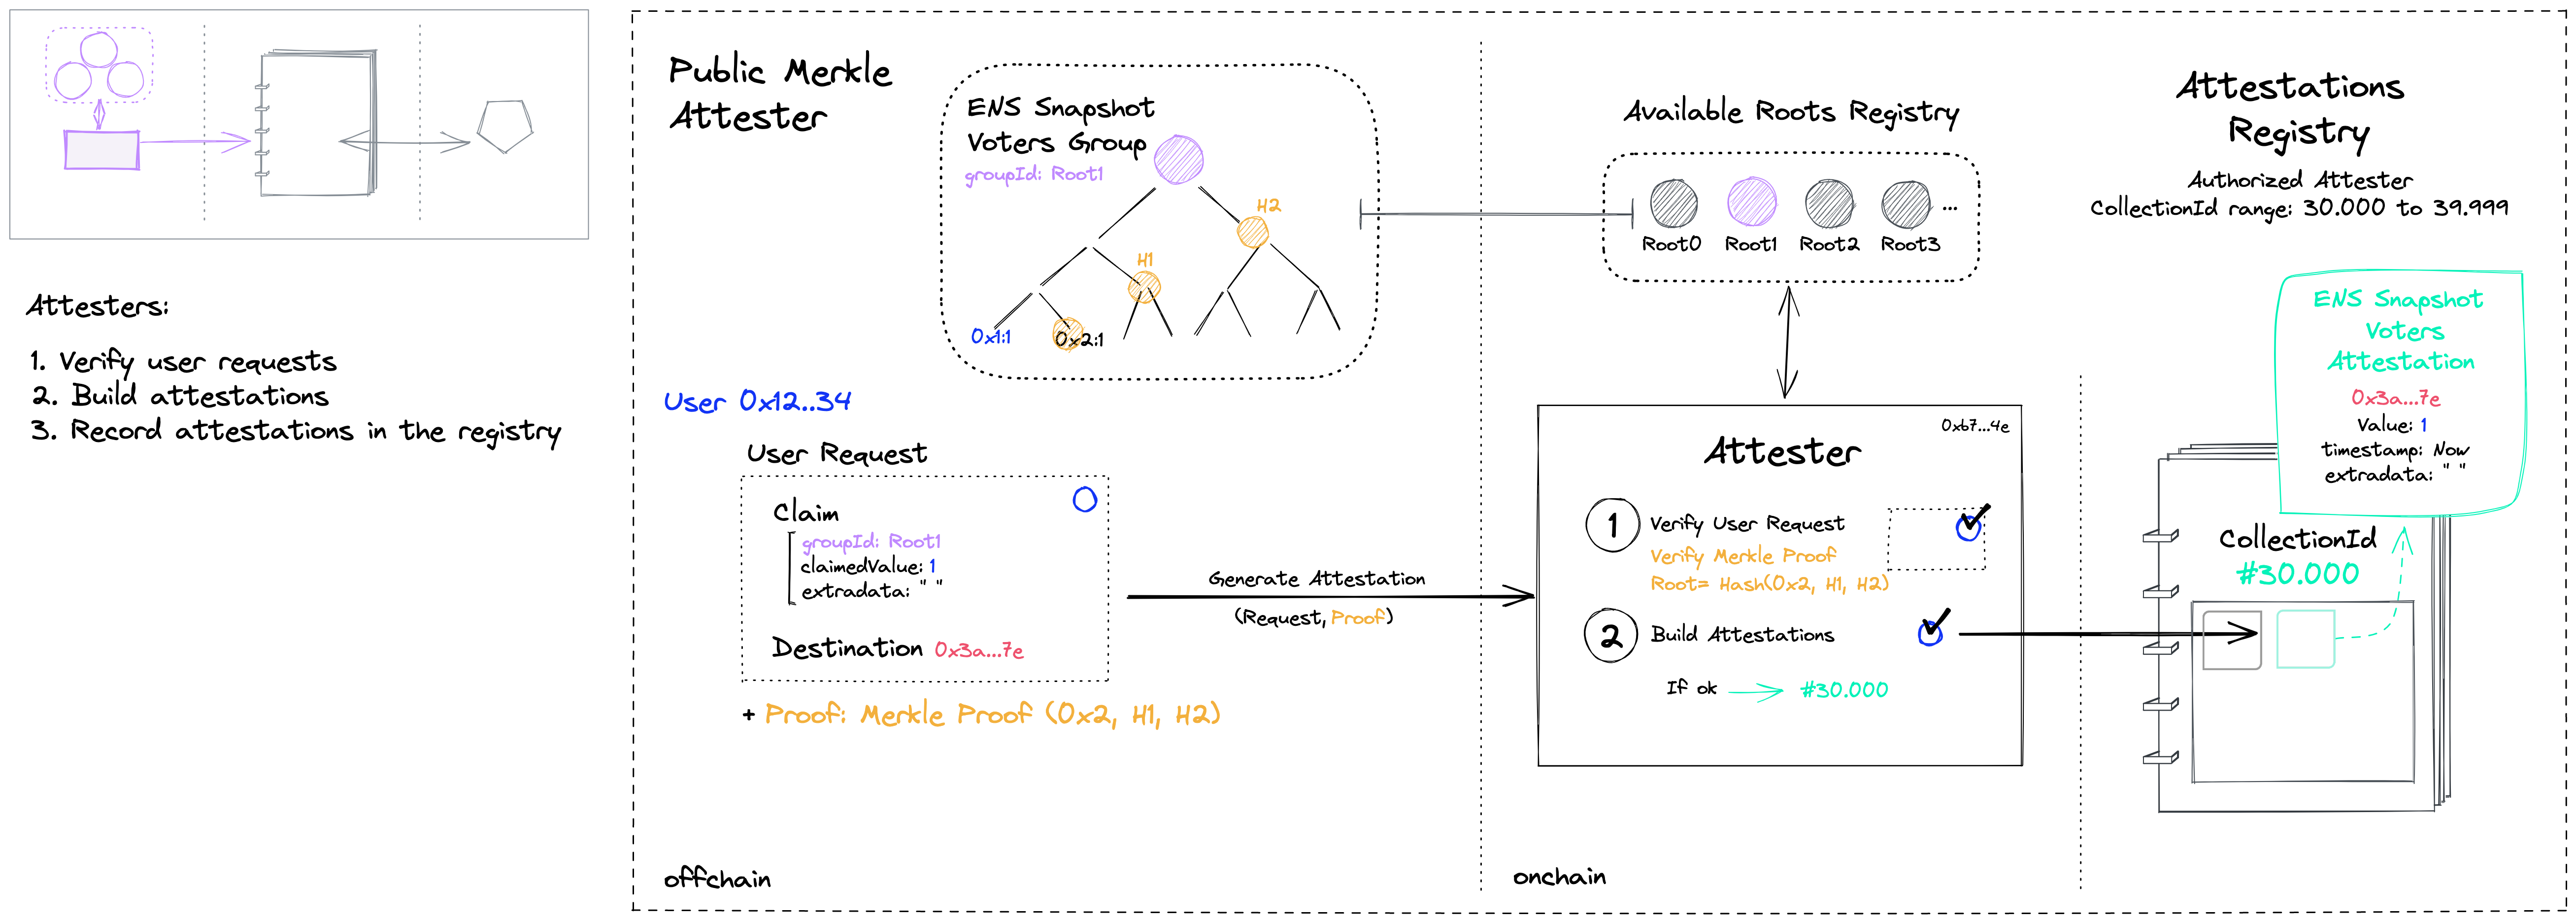
\includegraphics[width=1.\linewidth]{background/sismo2.png}
    \caption{Sismo: user claims their attestation.}
    \label{fig:sismo}
\end{figure}




\section{Blockchain basics}

The blockchain can be viewed as a replicated state machine. It means that  each time $t$ is associated with a global state which goes to the next state at $t+1$ with the state transition function. 

Here the state is for example account balances for bitcoin, the state transition function represented by the transactions, instructions to be executed to go to the next state.
In blockchain, the transactions for each state transition are placed in a new block, adding to the chain of blocks.
\begin{figure}[H]
\centering
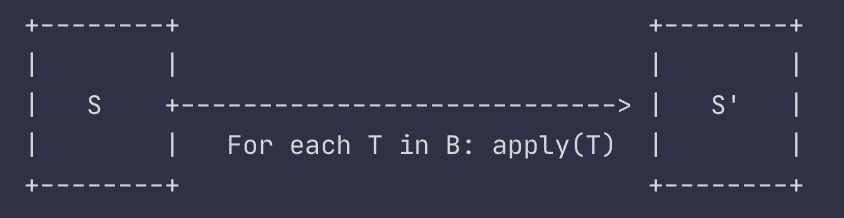
\includegraphics[width=0.6\linewidth]{background/state_transition.png}
    \caption{The state S transitioning to state S' by executing all transactions T from the block B}
    \label{fig:state_transition}
\end{figure}
Lastly, it is replicated across all the full nodes to ensure global consistency of the distributed ledger, meaning that the nodes on the network should agree on the blockchain state thanks to the consensus algorithm.

\subsection{The block}
So what is stored exactly in a block? 

Let's say for the moment that the bitcoin block consists of:
\begin{itemize}
    \item the hash of the previous block. You take the whole previous block and pass it to the hash function.
    \item the nonce resulting from the cryptographic puzzle. We'll talk about it later. 
    \item the list of transactions included in the block.
\end{itemize}
\begin{figure}[H]
    \centering
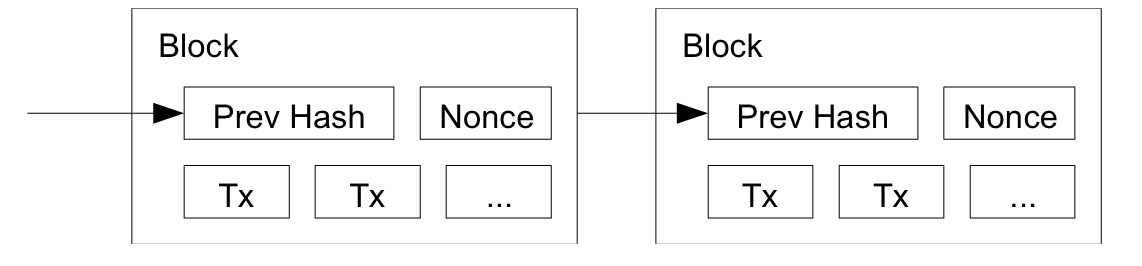
\includegraphics[width=0.6\linewidth]{background/block.png}
    \caption{A bitcoin block: the hash of the previous block, the nonce, and the list of transactions}
    \label{fig:block}
\end{figure}

This requires every node in the network to keep the list of transactions since 2009.

\subsection{Merkle tree of transactions}
In fact, the block is composed of the block header and the list of transactions. The block header contains this time the root hash of the transactions merkle tree.
The root hash is a summary of all the transactions happening during that period represented a merkle tree. For bitcoin, binary merkle tree are used for transactions, whereas in Ethereum, merkle Patricia trees are used to store transactions, state, receipts. 
\begin{figure}[H]
    \centering
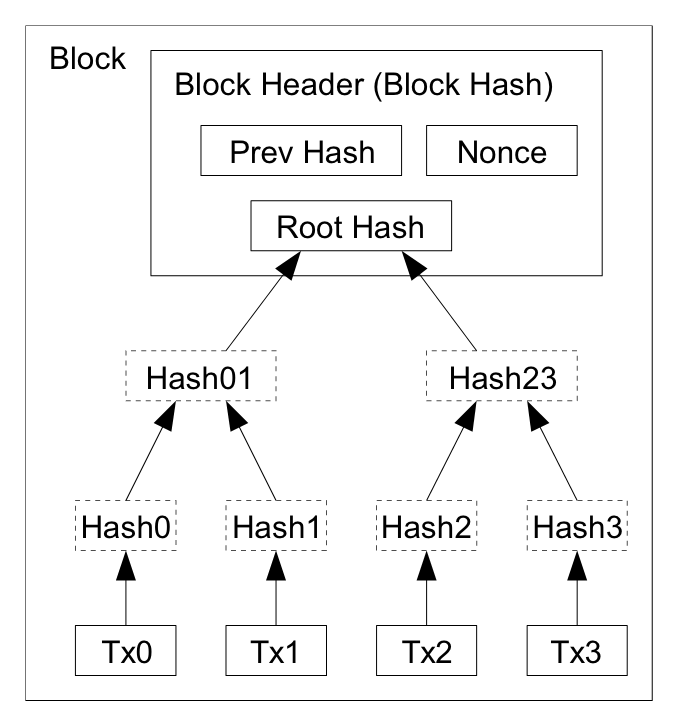
\includegraphics[width=0.4\linewidth]{background/blockmerkle.png}
    \caption{A Bitcoin\cite{Nakamoto..09} block}
    \label{fig:blockmerkle}
\end{figure}

\subsection{Single payment verification}
This allows two actors to emerge: \\
\textbf{The full node} stores all the full blocks, with the transactions. With this transactions, it can provide the proof of inclusion: the hashes required to prove a transaction is in a particular block. \\
\textbf{The light node } asks for the blocks headers to the full nodes of the network. Once he got the block headers, he can ask the full nodes of the network to provide a proof for the transactions is interested into. With the procedure described in \ref{merkle:inclusion}, the light node can verify that the transaction has indeed happened in the blockchain.

The light node is only storing the block headers, so even a phone can handle the amount of storage needed. This allows for example to verify with your wallet that a transaction has been executed  on your laptop without downloading the $\sim 500$GB of the blockchain.




\subsection{Security of light client}
\label{background:security}
We now share some security considerations about the block headers validity/finality. The light clients are able to verify the proofs of inclusion against the block header merkle root. \\But how can they trust this block header? Is it final ? Is it valid? 

\subsubsection{Proof of work}
In bitcoin and the proof of work, light clients ask the full nodes for the last block headers and select the longest chain. 
A block in bitcoin and in Proof of work contains a nonce (number generated once). This nonce represents the amount of work done by the validator to submit this block. 
Indeed the miners, full nodes with the ability to produce blocks, try to solve a cryptographic puzzle. This puzzle consists in testing all values of the nonce until they find one which make the hash of the block (including the nonce) starting with a certain number of zeros. 
In other words, they have to brute force a nonce such that the block hash meet the required level of difficulty: the number of zero. 
For example, if we ask the miners to find a hash of the block with only one zero, it'll be pretty easy. If we ask them to find a block hash with 10 starting zero, it'll probably be a lot more difficult. 

This nonce is the probabilistic guarantee that the block header is valid. The more blocks accepted (with a nonce then) after that block confirm that the transactions for this block and block header are valid and will not be reverted.

\subsubsection{Proof of stake}
If the proof of work relies on the amount of work for the security of the light client, the security of the proof of stake light client is a less obvious. 

As a proof of stake light client, we can get the genesis header and sync to the latest block header from it. But it's slow and unsafe because it's costless for a hacker to fork the network at some point and produce invalid blocks (long range attacks). 
Instead, the light client can ask a trusted source for header that is not in the unbounding window. It means that the trusted source, full node, can be slashed if it gives the light client fake block headers. The trusted source can be someone you know, a friend, a verified website for example.